% !TEX TS-program = pdflatex
% !TEX encoding = UTF-8 Unicode

% This is a simple template for a LaTeX document using the "article" class.
% See "book", "report", "letter" for other types of document.

\documentclass[11pt]{article} % use larger type; default would be 10pt

\usepackage[utf8]{inputenc} % set input encoding (not needed with XeLaTeX)

%%% Examples of Article customizations
% These packages are optional, depending whether you want the features they provide.
% See the LaTeX Companion or other references for full information.
\usepackage{url}
%%% PAGE DIMENSIONS
\usepackage{geometry} % to change the page dimensions
\geometry{a4paper} % or letterpaper (US) or a5paper or....
% \geometry{margin=2in} % for example, change the margins to 2 inches all round
% \geometry{landscape} % set up the page for landscape
%   read geometry.pdf for detailed page layout information

\usepackage{graphicx} % support the \includegraphics command and options

\usepackage{amsmath}
\usepackage{natbib}
% \usepackage[parfill]{parskip} % Activate to begin paragraphs with an empty line rather than an indent

%%% PACKAGES
\usepackage{booktabs} % for much better looking tables
\usepackage{array} % for better arrays (eg matrices) in maths
\usepackage{paralist} % very flexible & customisable lists (eg. enumerate/itemize, etc.)
\usepackage{verbatim} % adds environment for commenting out blocks of text & for better verbatim
\usepackage{subfig} % make it possible to include more than one captioned figure/table in a single float
% These packages are all incorporated in the memoir class to one degree or another...

%%% HEADERS & FOOTERS
\usepackage{fancyhdr} % This should be set AFTER setting up the page geometry
\pagestyle{fancy} % options: empty , plain , fancy
\renewcommand{\headrulewidth}{0pt} % customise the layout...
\lhead{}\chead{}\rhead{}
\lfoot{}\cfoot{\thepage}\rfoot{}

%%% SECTION TITLE APPEARANCE
\usepackage{sectsty}
\allsectionsfont{\sffamily\mdseries\upshape} % (See the fntguide.pdf for font help)
% (This matches ConTeXt defaults)

%%% ToC (table of contents) APPEARANCE
\usepackage[nottoc,notlof,notlot]{tocbibind} % Put the bibliography in the ToC
\usepackage[titles,subfigure]{tocloft} % Alter the style of the Table of Contents
\renewcommand{\cftsecfont}{\rmfamily\mdseries\upshape}
\renewcommand{\cftsecpagefont}{\rmfamily\mdseries\upshape} % No bold!


\newcommand*\mean[1]{\bar{#1}}

%%% END Article customizations

%%% The "real" document content comes below...

\title{Partially Observable Markov Decision Processes for Interactive Music Systems}
\author{Kevin Gibson, 1001319334}
%\date{} % Activate to display a given date or no date (if empty),
         % otherwise the current date is printed 

\begin{document}
\maketitle

\section{Overview}
Popular music has long relied on melody harmonies as a technique to distinguish vocal parts. Acts such as The Beatles, The Everly Brothers, and Simon \& Garfunkel featured multilayered vocal tracks to add complexity and richness to their songs. In bands such as Muse, The White Stripes, and Audioslave, guitar parts frequently use hardware to automatically generate harmonies on melodies, but the hardware lacks any sort of musical intuition and relies on simple pitch shifting to change the given input note \cite{whammy}. 

In recent years, a number of products have been released to allow the automatic creation of musically intelligent harmonies, following simple rules set by the user \cite{live5}. We present an implementation of a program to generate aesthetically pleasant harmonies to given input melodies. The system models a piece of music as a simplified partially observed Markov decision process (POMDP), where the actions made by the system have no effect on the state of the piece. A key-detection algorithm is implemented to generate a belief state, and we use MATLAB to create a prototype implementation. We propose several modifications to the existing system, as well as analyze the effectiveness of the program and look at limitations and extensions of the model. 

\section{System Model}
The project follows work from Martin et. al., with a slightly narrower focus, and some changes to the probabilistic model used \cite{martin2010}. A focus was made on using personal knowledge of music theory to improve the existing approach. The system is outlined in Figure \ref{fig:blockdiagram}, below. %Figure 1

\begin{figure}[h]
\centering
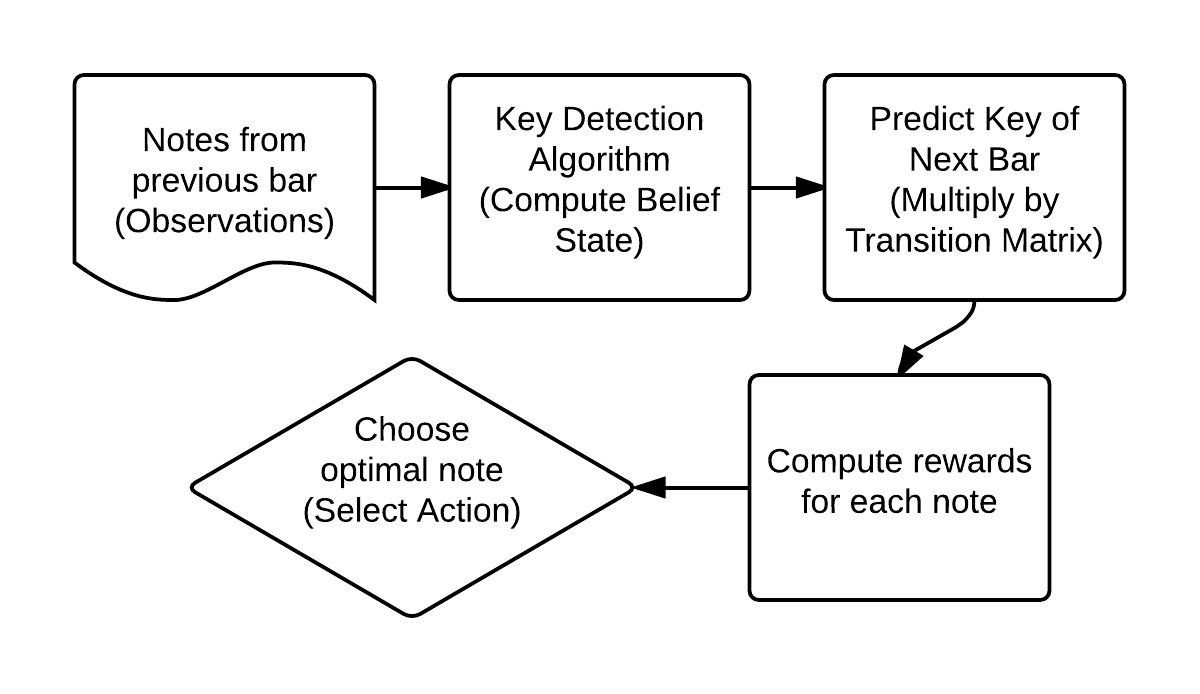
\includegraphics[resolution=300]{blockdiagram.png}
\caption{Block diagram showing the key components of the algorithm}
\label{fig:blockdiagram}
\end{figure}

The input to the system is a MIDI file containing an isolated melody track. MIDI is a widely used standard digital audio format, made up of note events triggered by a digital instrument such as a keyboard or synthesizer. The system is also initialized to know the tempo of the music, in order to determine how long a measure lasts. At the end of each measure, the key-finding algorithm generates a belief of what the key of that measure was based on the notes played. This is used to generate a belief state of the current measure by multiplying it by a transition matrix. The belief state is finally fed into a reward function, which returns a value for each note, based on the current belief state. The note with the highest reward is then chosen as the output note.

\subsection{Music Theory}
In order to understand the full system, a basic knowledge of western music theory is necessary. In contemporary western music, pitches are assigned to one of twelve different pitch classes related to the first 8 letters of the alphabet (see Figure \ref{keyboard}). Pitches which are given the same pitch class are a certain number of octaves apart, and sound harmonically pleasant when played together. More precisely, two pitches of the same class have frequencies that are integer multiples of each other.

\begin{figure}[h]
\centering
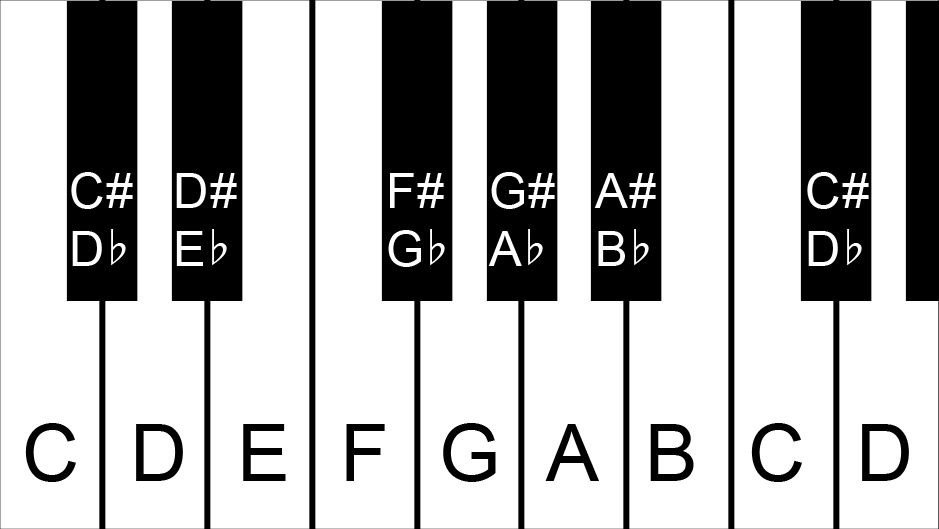
\includegraphics[width=0.6\textwidth]{keyboard.png}
\caption{A section of the keyboard with pitch classes labelled. Note the repeating nature of the pitch classes.}
\label{fig:keyboard}
\end{figure}

Another critical concept is the idea of a piece of music having a key, which could best be described as the tonal center of the piece. For our purposes, we consider there to be 24 keys, a major and a minor key for each of the 12 pitch classes. Each key has a scale of 7 notes associated with it, starting with the note the key is named after. We expect that most of the notes of a piece of music fall in the scale associated with that key, and it is on this assumption that we plan on generating pleasant harmonies for a given melody. The key of a piece of music can also change throughout the piece - J.S. Bach has several pieces which do not end on the same key as they start \cite{ged1979}.

While we can think of notes in terms of their absolute pitch class, we can also describe them relative to the current key. For example, if we have a piece of music in the key of F major, we can equally consider the note of C to be the fifth note of that key, as it is the fifth note occuring in the F major scale. Typically, roman numerals are used to indicate that notes are being discussed in relative terms, so we would say that in F major, C is the V. This is important, as we can define all our musical theory in relative, rather than absolute terms, giving us nice symmetry properties which we exploit. That is to say that patterns in music can all be definied in relative terms, and so when building probabilistic models of concepts such as key changes and common notes, we merely need to build the models relative to one key, and the same model can be quickly translated to all other keys. In blues music, for example, a common song structure is to play chords in a I-IV-V pattern, and so musicians can pick a key and immediately be able to play as an ensemble.

While there is a large body of musical theory to draw upon, this basic introduction should be enough to understand concepts in this project.
\subsection{POMDP Model}

%Review this section, and compare to the original paper - it has better notation and I can make sure i dont have errors.
The system uses a POMDP Model to represent the musical system, with the state of the POMDP representing the key of the piece being played at a given time. The discrete-time nature of the POMDP naturally conflicts with the continuous nature of music, so we treat a bar, or measure, of the piece as a discrete unit. Therefore, we assume that a piece has a single key inside a given bar. This generally agrees with music theory, except in cases where a drastic key change may be taking place. Since we cannot observe the key of a piece directly, we observe instead the notes being played, and use the key-finding algorithm to generate a belief state. 

Formally, we say that the piece at time $t_i$ exists in some state (key) $s_i$, and we have an observation of the system $o_i$. We use this to choose an action, $a_i$, which is a note played in bar $t_{i+1}$. Our action space is defined by the range of notes that can be played - in our case, we consider the 12 pitch classes as our action space, rather than the entire frequency range. Fortunately, our action space is not dependent on anything: we can choose to play any note at any time, simplifying the model. As well, there is no suggestion that the action actually has any impact on the next state, rather the stochastic process continues on indifferently. 

We denote the belief of the state at time $t_i$ as $b_i$, which is a vector with 24 entries, one for each major and minor key. We generate this belief from the observations of the previous bar: $b_i(s_i) = P(s_i | o_{i-1})$.  We define $P(s_i | o_{i-1})$ in two parts: the probability of being in a particular state given an observation of that state, $P( s_i | o_i)$, and the transition probability of moving from state $s_i$ to state $s_{i+1}$, $P(s_{i+1} | s_{i})$. By the chain rule, we have
\begin{align*}
P(s_i | o_{i-1}) &= \sum_{s_{i-1} \in S} P(s_i | s_{i-1}, o_{i-1}) P( s_{i-1} | o_{i-1}) \\
&= \sum_{s_{i-1} \in S} P(s_i | s_{i-1}) P( s_{i-1} | o_{i-1})
\end{align*}
so we see that we can use the standard concepts from POMDPs of transition matrices to help generate our belief state. We assume that the note played by our system has no impact on the transition probability, as in our simple implementation we are dealing with pre-recorded melodies. Thus our transition depends entirely on the previous state. In our system, the transition matrix is hand-tuned, relying on the symmetric properties of music to allow us to define the entire $24\times24$ matrix as shifted versions of a single 24-element vector. 

Finally, we have a reward function $r(a_i, s_i)$, which returns a value representing the desirability of playing note $a_i$ in a given key $s_i$. Essentially, it is a representation of the musical properties of a note in that key, with higher values corresponding to a more musically pleasing fit in that key. By tweaking the transition matrix and the reward function, we can in theory drive different behaviours suitable for different genres of music.

To determine what note is ideally played, it is necessary to compute the optimal value function and the corresponding policy. In general, this problem is computationally hard and not suitable for real-time systems; however, in this case it is suitable to use a finite horizon approach with a single stage cost-to-go function, making solving trivial. This is the case because there is no limitation on the notes we can play - our action space is the complete set of notes, regardless of our previous action or current state. As well, since our reward function is simply a function of the current state and does not depend on past actions, the optimal policy in this case would be the same regardless of our choice of cost horizon. If we were to modify our reward function to depend on our action history, this would not be the case, and more care would have to be made with regards to our policy finding.

\subsection{Key-Finding Algorithm}
In order to generate a belief state, we must have some model for how certain notes being played correspond to a musical key. The original work uses the Krumhansl-Schmuckler Key-Finding Algorithm, which relies on the idea of calculating correlations between note inputs and key profiles to estimate a key \cite{clk1990}. %Cite Krumhansl-Schmuckler
For each major and minor key, there is a provided key profile vector of 12 values, loosely representing the likelihood of the 12 pitch classes being played in that key. To determine the key of a given segment of music, we first construct an input vector consisting of 12 values representing the durations of each pitch class in that segment. The correlation between a given input vector, $x$, and a given key-profile, $y$, is computed as
\[
	r= \frac{\sum(x-\mean{x})(y-\mean{y})}{(\sum(x-\mean{x})^2\sum(y-\mean{y})^2)^{1/2}}
\]
where $\mean{x}$ is the average of the input vector values, and $\mean{y}$ is the average key-profile value for that given key. Computing the correlation for all 24 key-profile vectors, we say that the key-profile which gives the highest correlation gives us the preferred key. \\
Temperley provides us with a few improvements to the original key-finding algorithm, both with improved key-profile vectors, and with what he calls a ``flat-input'' approach \cite{temperley1999}. The new key profiles are a minor change, but by ensuring that the mean for all the profiles is the same, computing the correlations is slightly simplified. The ``flat-input'' approach simply changes the input vector to be a binary vector, with a given value being 1 when a note appears in a segment of music, and 0 when it does not. While this seems like it should reduce the information gleaned from a section, through testing it appears to increase accuracy over a number of sample pieces.

%Example of converting music to note vectors
\begin{figure}[h]
\centering

\includegraphics[width=0.4\textwidth]{emaj.png}
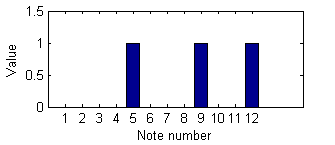
\includegraphics[width=0.4\textwidth]{emajvector.png}
\caption{A piece of music showing an E major chord, and the corresponding ``flat-input'' vector. Pitch classes are numbered from 1-12, with 1 corresponding to C.}
\label{fig:inputvector}
\end{figure}

In order to get a probabilistic belief state from a given key, the original paper generates estimates for the probability of making an observation given a key, and uses this as their belief state of the actual key \cite{martin2010}. Using the key-profiles as a discrete probability distribution, they generate a large number of 16-note sequences, and run the key-finding algorithm on each. By knowing what key-profile was used to generate the sequence and comparing this to the key that was output by the key-finding algorithm, they find a belief state for any given output of the key-finding alrogithm. However, in doing so, they discard any information that may be learned from the specific note information. From a strictly information theoretic standpoint, it would be better to use the correlations output by the algorithm directly to generate a belief state. To do this, we simply scale the correlations generated by each input so that all values lie between 0 and 1, and so that the sum of all the correlations is 1. 

\section{Implementation}
We create an implementation of the system in MATLAB. We use Ken Schutte's library to read and write MIDI files, and the built in matrix functions to let us quickly create a prototype and perform analysis. While the structure of the program would allow it to run in real-time, by using pre-recorded MIDI files the code was run offline, allowing for faster iteration times. We also made several modifications to the prior work, with the goal of generating more musical output.

The first modifications were made to the key-finding algorithm, as described above. By scaling the output, we were able to generate a belief state directly from the given correlations. This was done by first setting the probabilities of all keys with negative correlations to 0, then multiplying the remaining correlations such that they summed to 1. The setting of negative correlations to 0 was a design choice made after finding that simply shifting and scaling the correlations led to innaccurate note choices, giving small but non-zero probabilities to a large number of keys. Since the number of keys with negative correlations was large, it occassionally led to these keys having undue influence on the note chosen, despite their individual unlikelihood. A comparison of the three approaches can be seen in Figure \ref{fig:belief}. Note that all three approaches place the largest probability on the same value, but the new approach has large probabilities on other likely keys which are note as present in the original approach.

%Need figure showing a piece of music, with the belief state generated from the three different methods
\begin{figure}[h]
\centering

\begin{tabular}{cc}

\multicolumn{2}{c}{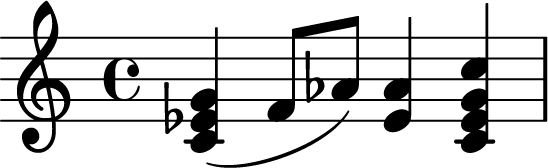
\includegraphics[width=0.4\textwidth] {belief.png}}\\
\multicolumn{2}{c}{Input bar}\\
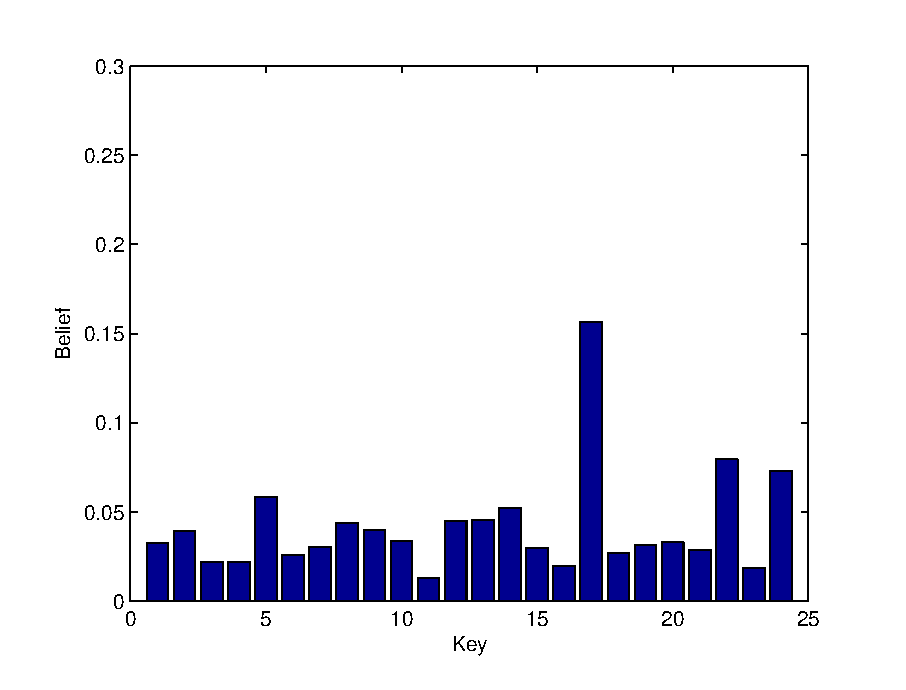
\includegraphics[width=0.4\textwidth]{belieforiginal.eps} & 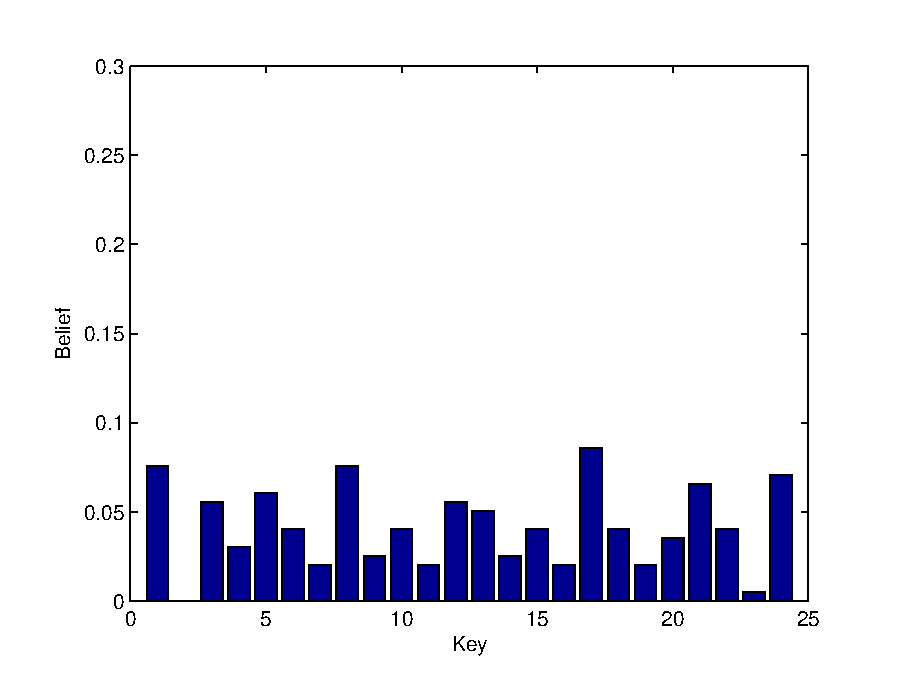
\includegraphics[width=0.4\textwidth]{beliefcorrelation.eps}\\
(a) Original approach & (b) Scaled correlations \\
\multicolumn{2}{c}{ 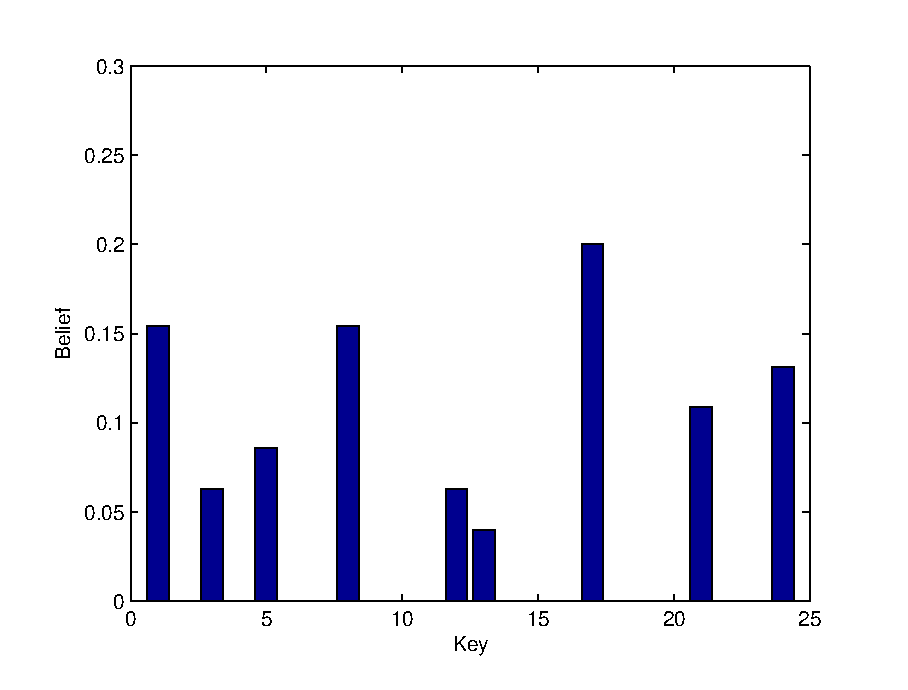
\includegraphics[width=0.4\textwidth]{beliefnew.eps}} \\
\multicolumn{2}{c}{(c) New approach}
\end{tabular}
\caption{Comparison of belief vectors generated by the three different methods.}
\label{fig:belief}
\end{figure}


The next, more important modifications were to the transition matrix and the reward function. The transition matrix was constructed from a hand-tuned 24-element vector,with values corresponding to the 24 major and minor keys. In the original work, the transition probabilities were quite simple: a high probability was given to staying in the same key, and an equal probability was given to changing to any other state. By looking at patterns in popular and classical music, it is obvious that not every key change is equally likely, and our transition vector was crafted to reflect this. Essentially, it was crafted to represent the likelihood of going from a given key to any other key, based on personal knowledge of music theory and composition. A higher likelihood was given to changing to a key that has its chord present in the scale of the current key. For example, since the C major scale contains the notes of the G major, A minor, and F major chords, they all have high probabilities in the transition. As in the original, the highest probability is given to staying in the same key, reflecting the relative rarity of key changes in music. The next highest probabilities were given to the major IV, major V, and minor vi keys, as they are common key changes in popular music. Using the relative nature of music, we are able to use this vector for all major and minor keys, taking care to shift everything to be in relative pitch terms, rather than absolute.

 The reward function is again crafted by hand, and differs significantly from the original work. The original reward function simply applies a positive reward value $a$ for every note that occurs in the scale of the key, and a negative reward $-a$ for any note not in the scale of the key. This oversimplification can lead to unusual choices, as in most popular music certain notes are much less likely to occur. Fortunately, we already have a representation of the likelihood of each note in a given key, in the form of the key-profiles from the key-finding algorithm. We use these values directly as our rewards, as they have already been tested and are representative of understood music theory.

\section{Evaluation}
%Can't do this right now - need data!
%Explain the table and how we evaluate our approach.
In order to evaluate the success of our approach, a method for quantifying the performance is necessary. This is difficult as it clashes with the highly personal nature of music; however, we can come up with some numbers that at least help compare different approaches. We do this by using the key detection algorithm to determine the key of each bar, and comparing it to the note chosen to be played in that bar. Essentially, we compare the notes chosen based on information from the previous bar to our best estimate of the key based on information of the current bar. We use the key-profile vectors to assign a reward to the notes chosen by the two methods: the original work, and the new approach using the modifications to the key detection and reward function. For key detection, we choose the key which gives the highest correlation value, and ignore the others. Running this evaluation on a variety of pieces, we see that the modifications proposed here to result in a significant improvement in scores - essentially, the new approaches choose notes that are more likely to ``fit-in'' with the other notes in the bar. Note that this method is not suitable for providing a raw evaluation of the performance, merely to compare two methods as a benchmark.

\begin{table}[h]
\begin{tabular}{@{}lll@{}}
\toprule
                                      & Our Approach & Old Approach \\ \midrule
``Jesu, Joy of Man's Desiring" - J.S. Bach         & 15.9583      & 9.9583       \\
``Fur Elise" - Beethoven                          & 196.6667     & 148.6667     \\
Brandenburg Concerto No 2, Movement 1 - J.S. Bach & 552.2500     & 379.2500     \\
``All My Lovin'" - The Beatles         & 217.5417     & 143.5417     \\
``A Hard Day's Night" - The Beatles         & 188.5000     & 93.5000      \\ \bottomrule
\end{tabular}
\caption{Total reward scores for a variety of songs, comparing the modified method presented here to the original work.}
\label{table:scores}
\end{table}

As well as the above quantitative approach, a significant amount of qualitative evaluation was done to determine the success of the algorithm. In general, it was found that the system produced pleasant, natural sounding choices for notes. Most of the times when notes sounded ``off'' was when a key change occurred partway through a measure, and it was for a brief period of time. While it is still likely not good enough to be used in live music situations, it certainly has promise as another tool in algorithmic music composition.

\subsection{Limitations}
%Need to discuss output rhythms, choosing an octave, etc.
The system as it stands has many limitations which will need to be addressed in the future. The most obvious is that the system does not have any system in place to output rhythms, and so in its current incarnation follows the input rhythm. While this is okay for situations where harmonizing an existing melody is the goal, it means that it is not possible to use this approach to generate a melody from a rhythm part, such as generating a synthesized solo on top of a guitar track. 

Another, more serious limitation is that the basic reward function described here takes no consideration of the action history, and so tends to repeat itself. This is rather challenging to fix - on the one hand, too much repetition leads to boring music, and it is easy to modify the reward function to punish repetition; on the other hand, music without repetition seems random and hard to follow along with. The robust solution to this would require a significantly more complicated reward scheme, which would likely necessitate a discounted cost approach to finding a solution, leading to increased computational costs.

\section{Future Work}
While the current implementation is interesting, there is a lot of room for expansion and improvement. Perhaps the most obvious first step would be to investigate data-driven ways of creating the transition matrix. One possible way to do this would be through the use of machine learning algorithms, although an even simpler unsupervised approach may be sufficient. If a large corpus of songs is available, it would be a simple matter of running the key-finding algorithm on each bar, assuming the strongest correlation indicates the key. By counting the different key transitions between bars it would then be trivial to generate a distribution from these numbers. 

There is also plenty of room for improvement with regards to the reward function. More complex functions could take into consideration heuristics to avoid note repetition, encourage certain note sequences, or even promote certain melodic motifs that repeat throughout the piece. In order to do this, it would be necessary to switch to a discounted cost or larger finite horizon value function, which significantly increases computational complexity. This may be more suitable to generating melodies offline, for use in algorithmic composition programs. A more complicated improvement would be to learn the reward function, by studying melodies over harmony parts.

Another place for future work is in switching away from MIDI input and using raw audio data. This would be a fairly simple change, as there are already a number of algorithms for determining the note from a sound sample using Fourier analysis \cite{gerhard2003}.
This would simply be a new front end to the existing system, but may require dedicated hardware to get working in real time. 

\section{Conclusion}
We have presented a method for generating a harmony of a given piece of music, using a POMDP model and the Krumhansl-Schmuckler Key-Finding algorithm. We implemented a previous method and showed minor changes that can increase performance, and evaluated both methods on a range of music pieces. While simplistic, the effectiveness of this proof of concept shows that there are ways to improve by applying existing techniques, and we offer several directions for future work.

\bibliographystyle{plain}
\bibliography{project}

\end{document}
